\documentclass{ctexart}

\usepackage{ctex}
\usepackage{tikz}
\usetikzlibrary{calc,positioning,shapes.geometric}
\usepackage{url}
\usepackage{graphicx}
\usepackage{float}
\usepackage{xcolor}
\usepackage{color}
\usepackage{amsmath}
\usepackage{amsthm}
\usepackage{amssymb}
\usepackage{mathrsfs}
\usepackage{caption}
\usepackage{subfigure}
\usepackage{framed}
\usepackage{booktabs}
\usepackage{makecell}
\usepackage{geometry}
\usepackage{wrapfig}
\usepackage{abstract}
\usepackage{algorithmicx}
\usepackage[ruled]{algorithm}
\usepackage{algpseudocode}
\usepackage{setspace}
\usepackage{bm}
\usepackage{cite}
\usepackage{array}
\usepackage{textcomp}
\usepackage{listings}

\definecolor{shadecolor}{rgb}{0.93,0.93,0.93}
\usepackage{geometry}
\geometry{right=2.5cm,left=2.5cm}

\newtheorem{theorem}{定理}

\pagenumbering{arabic}

\begin{document}
\begin{sloppypar}
\title{\vspace{-3cm} \textbf{数值分析第二章编程作业报告}}
\author{刘陈若\;$3200104872$\\信息与计算科学2001}
\date{}

\maketitle

\section*{程序编译和运行说明}
本次项目作业采用Makefile文件对编译进行统一管理。具体地,在Makefile所在目录下输入\verb|make|
即可完成编译,得到problem\verb|B|-problem\verb|E|的可执行文件\verb|B|,\verb|C|,\verb|D|,\verb|E|。分别对其进行运行,即可得到各小题的输出结果,具体内容将在下一节中按问题顺序分别作出说明。

\section*{程序运行结果及简要分析}
\subsection*{Problem A}
问题A没有数值输出,其具体的要求都已经全部在头文件\verb|interpolationsolver.h|中得到实现。

具体来说,头文件首先定义了Function类和Interpolation类,分别对不同类型的函数以及插值公式进行抽象。除了一般化的函数外,Newton polynomial和Hermite polynomial类对Function类进行继承。通过运算符()的重载,只需给出插值多项式所有$\pi_k(x)$前的系数$a_k$,即可唯一表示对应的函数。

而系数的确定将由Interpolation类完成。Interpolation类派生出的Newton Formula和Hermite Formula类分别根据差商计算公式递推得到所有系数$a_k$,得到相应的Newton polynomial和Hermite polynomial,并且通过solve()函数(以及Hermite polynomial特有的solvediff()函数)分别返回插值函数在任意一点的函数(以及导数)值。

\textbf{有两点需要格外注意}。首先,Newton Formula和Hermite Formula类的具体对象构造方式并不相同,Newton Formula需要给出的是带插值函数和插值点的位置,而Hermite Formula需要给出的是插值点位置和插值点的函数(及其导数)值。其次,根据题目要求,希望实现的是给出一个能够返回插值多项式任意一点函数值的接口,也就是说,希望能把具体的系数$a_k$封装在类内,而不是返回插值函数的具体表达式交由用户进行函数值计算。因此,虽然设计了Get coef()函数返回插值多项式的相应系数,但除了本实验报告的必要展示之外,应尽量避免使用该函数。

\subsection*{Problem B}
问题B中,首先对$n = 2,4,6,8$,分别利用函数$f(x) = 1/(1+x^2)$在插值点$x_i = -5 +i/n$,$i = 0,1,\dots,n$的值进行插值,然后对不同n的值对应的插值函数进行描点采样,并将采样数据存储至\verb|probB_result.txt|文件后导入Python绘制出其图像,和真实的$f(x)$图像比较得到下图。
\begin{figure}[H]
\centering
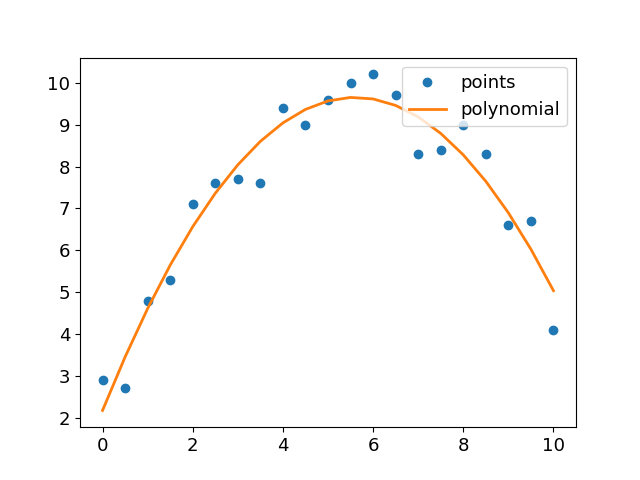
\includegraphics[height=6.8cm,width=9.5cm]{Figure_1.png}
\label{Fig1}
\end{figure}

从图中可以看出,对于$f(x)$采用等间距节点插值会产生明显的Runge现象,随着$n$的增加插值函数并未达到更好的拟合效果,并且在区间端点处产生了更为剧烈的振荡。

\subsection*{Problem C}
问题C中,首先对$n = 5,10,15,20$,分别利用函数$f(x) = 1/(1+25x^2)$在Chebyshev多项式的零点$x_i =\cos \frac{2i-1}{2n}\pi$,$i = 1,2,\dots,n$的值进行插值,然后对不同n的值对应的插值函数进行描点采样,并将采样数据存储至\verb|probC_result.txt|文件后导入Python绘制出其图像,和真实的$f(x)$图像比较得到下图。
\begin{figure}[H]
\centering
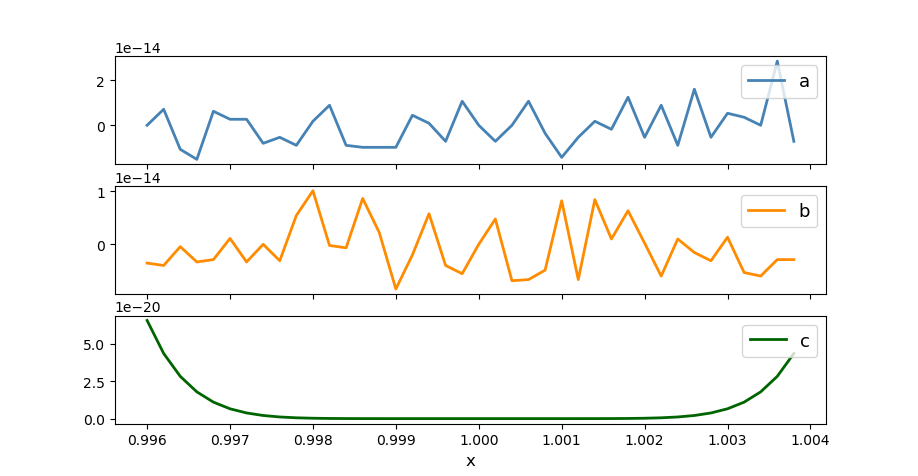
\includegraphics[height=6.8cm,width=9.5cm]{Figure_2.png}
\label{Fig2}
\end{figure}

从图中可以看出,对于$f(x)$,将Chebyshev多项式的零点作为节点进行插值时,随着$n$的增大,多项式函数对原函数具有更好的近似效果,有效地避免了插值函数振荡的问题。

\subsection*{Problem D}
\subsubsection*{(a)} 如果记距离$D$关于时间$t$的函数为$D=f(t)$,根据题意有
\begin{equation}
\begin{split}
    f(0)=0,\quad f'(0)=75,\quad f(3)=225,\quad f'(3)=77,\quad f(5)=383 \\
    f'(5)=80,\quad f(8)=623,\quad f'(8)=74,\quad f(13)=993,\quad f'(13)=72
\end{split}
\end{equation}
将这些插值点和对应数据输入进行Hermite插值后,对其在$t=10s$处的距离和速度进行预测,程序有如下输出:
\begin{shaded}
\begin{verbatim}
The car's distance at t = 10s is 742.503 feet
The car's speed at t = 10s is 48.3817 feet/s
\end{verbatim}
\end{shaded}
也即,根据插值结果,在$t=10s$处的距离和速度分别为742.503 feet和48.3817 feet/s.
\subsubsection*{(b)}
通过对得到的Hermite插值函数的导数利用solvediff()函数进行描点采样,并将采样数据存储至\verb|probD_result.txt|文件后,导入Python可以绘制出汽车速度随时间的图像如下图所示。
\begin{figure}[H]
\centering
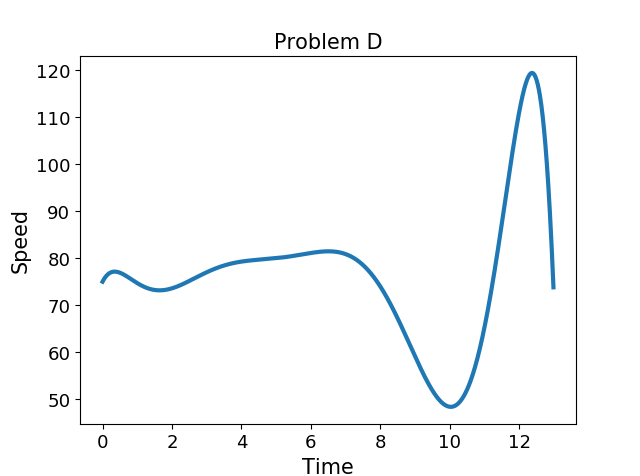
\includegraphics[height=6.2cm,width=8.5cm]{Figure_3.png}
\label{Fig3}
\end{figure}
从中可以很直观地看出,当$t$在$12s$左右时,根据图像此时汽车速度将远远超过$55$$mi/h$。事实上,如果以$0.01s$为间隔进行等间隔采样,可以近似得到汽车在观测过程中的最大速度为:
\begin{shaded}
\begin{verbatim}
The max speed during the observation is 119.417 feet per second
\end{verbatim}
\end{shaded}

\subsection*{Problem E}
\subsubsection*{(a)}
使用Newton公式对两类样本分别进行插值,利用Get coef()函数得到两个插值函数的系数分别为:
\begin{shaded}
\begin{verbatim}
The Coefficients of curve for Sp1 are: 6.67 1.77167 0.457833 -0.124778 0.013566
-0.000978085 4.1477e-05 
The Coefficients of curve for Sp2 are: 6.67 1.57167 -0.0871667 -0.0152729
0.00257908 -0.000204804 8.6768e-06 
\end{verbatim}
\end{shaded}
因此,两类种群的Average weight curves分别为
\begin{equation}
\begin{split}
    p_{Sp1}(x) = 6.67\pi_0(x) + 1.77167\pi_1(x) +0.457833\pi_2(x) -0.124778\pi_3(x) \\
    + 0.013566\pi_4(x) -0.000978085\pi_5(x) + 4.1477*10^{-5}\pi_6(x) \\
    p_{Sp2}(x) = 6.67\pi_0(x) + 1.57167\pi_1(x) -0.0871667\pi_2(x)  -0.0152729\pi_3(x) \\
    + 0.00257908\pi_4(x) -0.000204804\pi_5(x) + 8.6768*10^{-6}\pi_6(x)
\end{split}
\end{equation}

直观来看,对函数进行描点采样,并将采样数据存储至\verb|probE_result.txt|文件后,导入Python后绘制出如下所示函数图像。图像的简单分析将在(b)中一并进行。
\begin{figure}[H]
\centering
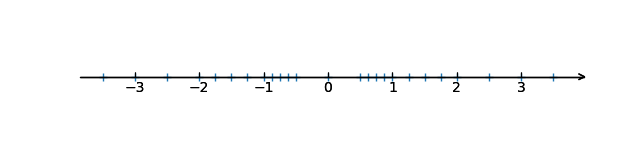
\includegraphics[height=6.5cm,width=9.2cm]{Figure_4.png}
\label{Fig4}
\end{figure}

\subsubsection*{(b)}
根据(a)中的插值函数,可以得到$15$天后,也就是第$43$天时两类样本的Average weight,以及样本在$28$-$43$天之间的平均重量曲线如下所示。
\begin{shaded}
\begin{verbatim}
Average weight of Sp1 after another 15 days is: 14640.3
Average weight of Sp2 after another 15 days is: 2981.48
\end{verbatim}
\end{shaded}
\begin{figure}[H]
\centering
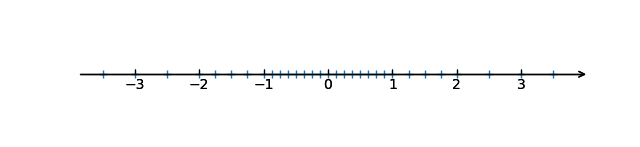
\includegraphics[height=6cm,width=9.2cm]{Figure_5.png}
\label{Fig5}
\end{figure}
显然这样的结果是与直觉相违背的。结合(a)中的图像,我们可以得到如下结论:当插值点无法自主决定时,可能会产生Runge现象导致插值函数与真实函数在观测区间内发生较大差异;此外,插值函数对观测区间外的函数值并不一定具有好的预测效果。

\end{sloppypar}
\end{document}
